% simdoc.tex V3.0, 30 March 2010

\documentclass[12pt, times]{simauth}

\usepackage{moreverb}

%\usepackage[T1,mtbold]{mathtime} % commented by ShareLaTeX Team because of compilation errors

\usepackage[
%dvips, % commented by ShareLaTeX Team because of compilation errors
colorlinks,bookmarksopen,bookmarksnumbered,citecolor=red,urlcolor=red]{hyperref}

\usepackage[utf8]{inputenc}
\usepackage[T1]{fontenc}
\usepackage[spanish]{babel}
\usepackage{upquote}
\usepackage{epigraph}
\usepackage{makeidx}
\usepackage{framed}
\usepackage{pgf}
\usepackage{tikz}
\usepackage{amsmath,cases,mathtools}
\usepackage{amsthm}
\usepackage{array}
\usepackage{MnSymbol,wasysym}
\usepackage[pdftex,active,tightpage]{preview}
\usetikzlibrary{babel}
\usetikzlibrary{arrows,automata,positioning}
\graphicspath{ {images/} }
\usepackage{pgfplots}
\usepackage[lined,boxed,commentsnumbered]{algorithm2e}
\usepackage{calligra}
\usetikzlibrary{er}


\def\volumeyear{2010}

\SetKwProg{Fn}{Function}{}{}

\begin{document}

%\runninghead{A.~N.~Other}

\title{
    {\fontfamily{ppl} \fontsize{30}{1} \selectfont{
        SOA: Apuntes 13 de Marzo 2017 }
    }
}

\author{
    {\fontfamily{ppl} \fontsize{14}{1} \selectfont{
        Carlos Martín Flores González \\
        Carné: 2015183528}
    }
}

%\address{John Wiley \& Sons, Ltd, The Atrium, Southern Gate, Chichester,
%West Sussex, PO19~8SQ, UK}
%
%\corraddr{Journals Production Department, John Wiley \& Sons, Ltd,
%The Atrium, Southern Gate, Chichester, West Sussex, PO19~8SQ, UK.}

%\begin{abstract}
%This paper describes the use of the \LaTeXe\ \textsf{simauth.cls}
%class file for setting papers for \emph{Statistics in Medicine}.
%\end{abstract}

%\keywords{class file; \LaTeXe; \emph{Statist.\ Med.}}

\maketitle

\tableofcontents

\section{Administrativo -- Recordatorios}

\subsection{Quiz \#4}
\begin{enumerate}
    \item Los últimos \emph{CPU-burst} de un un proceso han sido 15ms-40ms-3ms-17ms. Si el promedio del sistema es de 30ms y se usa un parámetro de $\alpha = 0.5$. ¿Cuál es la predicción del siguiente \emph{CPU-burst}?
    \item Explique el problema de ``Inversión de Prioridades''.
    \item Explique el algoritmo de \emph{Lottery Scheduling}.
\end{enumerate}

\subsection{Forro para exámen}
El ``forro'' oficial para los exámenes: una página tamaño carta escrita a mano. 

\subsection{Resúmenes para la próxima semana}
\begin{enumerate}
    \item 0311
    \item 0320 $\rightarrow$  Este se va a exponer
    \item 0401
    \item 0402
    \item 0406
\end{enumerate}
También se va a exponer el artículo 0608.

\newpage
\section{Monitores de Máquinas Virtuales (VMM)}
Un monitor de máquinas virtuales\footnote{También se les llama Hipervisores} (VMM) es un sistema de software que particiona una máquina física en múltiples máquinas virtuales. Tradicionalmente los VMMs han creado réplicas precisas del la máquina física que las soporta. A través de emulación, los VMMs soportan la ejecución de sistemas operativos invitados(\emph{guest}) como Windows o Linux sin necesidad de modificadiones \cite{whitaker}.


\paragraph{Escenario:}
se desea simular una arquitectura en otra, por ejemplo ARM en x86. ¿Cómo sería este programa? 

El programa sería un intéprete, se escribiría un ciclo de \texttt{FETCH}. Hay que tomar como entrada el código de una operación (por ejemplo un \texttt{shift} a la izquierda) y hacer algo  en lenguaje C que haga lo mismo.

Probablemente en el corazón de este programa habría un \texttt{switch/case} muy grande con todos los códigos de operacion y su respectiva interpretación.


\begin{algorithm}[H]
\DontPrintSemicolon
            \Switch{código\_operación}{
                \uCase{SHL:}{
                    \texttt{...} \;
                    \texttt{...} \;
                    \texttt{break;}
                }
                \uCase{ADD:}{
                    \texttt{...} \;
                    \texttt{...} \;
                    \texttt{break;}
                }
                \texttt{...} \;
                \texttt{...} \;
                \texttt{...} \;
            }
\end{algorithm}


En ensamblasor el ejercicio sería relativamente similar, en una parte está el bloque que hace el \texttt{shift} a la izquierda en ARM y luego implementando varias instrucciones \emph{jump}\texttt{(jmp)}, se podría llegar a la rutina de conversión deseada. 

\paragraph{¿Y si las dos arquitecturas son muy diferentes?} La simulación de cada instrucción sería muy grande y complicada.

\paragraph{¿Qué tal si no son tan diferentes?} El conjunto de instrucciones se hace más pequeño.

\begin{center}
\framebox[1.1\width]{Arquitecturas más parecidas = simulación más fácil y corta} \par
\end{center}

\paragraph{¿Y si hubiera que hacer un simulador de x86 en x86?} Se usaría la misma instrucción para simular la instrucción del otro lado.

\paragraph{¿Cómo hacer un simulador de una arquitectura en ella misma?}
\begin{itemize}
    \item Se deja que corra sobre el mismo hardware.
    \item Todo lo que ocurre tiene que ser aislado
    \item Tiene que ser perfecta, cualquier software que corra en el hardware real tiene que correr en la simulada.
    \item \textbf{El verdadero reto en máquinas virtuales es ejecutar una arquitectura en sí misma.}
    \item La protección al final es un concepto de hardware.
    \item El sistema operativo al final lo que hace es restringuir la simulación porque restringue al programa que se está ejecutando.
    \item Esta idea nace a partir de los años 70s.
    \item Tuvo mucha actividad al principio y luego pasó de moda
    \item Se considero algo muy académico, pero en realidad el concepto es muy elegante e interesante en sistemas operativos.
\end{itemize}

\subsection{¿Cómo escribir un VMM?}

\begin{center}
\begin{tikzpicture}
[every entity/.style={fill=blue!20,draw=blue,thick},
every relationship/.style={fill=orange!20,draw=orange,thick,aspect=1.5}]
\node[entity] (hw) at (0,1) {Hardware};
\node[entity] (vmm) at (0, 2) {VMM}
child {node[attribute] at (0, 3) {$H'$}
    child {node[attribute] at (0, 3) {$OS'$} }
}
child {node[attribute] at (0,3) {$H'$}
    child {node[attribute] at (0,3) {$OS''$} }
}
child {node[attribute] at (0,3) {$H'$}
    child {node[attribute] at (0,3) {$OS'''$} 
        child {node[attribute] at (0,3) {$P_1$} }
        child {node[attribute] at (0,3) {$P_2$} }
    }
};  
    edge (hardware)
    edge (vmm);
\end{tikzpicture}
\end{center}

\begin{itemize}

\item Hay un hardware que es el verdadero.
\item Sobre ese hardware va a correr un software, el VMM
\item Este software va a crear varias máquina virtuales 
\item \underline{Requisitos:}
    \begin{itemize}
        \item Los $H'$ son idénticos al hardware que está debajo del VMM.
        \item Cualquier software que corre en el hardware real debería de correr en las virtualizadas.
        \item Un software que interesaría que corriera en $H'$ sería un sistema operativo.
        \item Podrían ser diferentes sistemas operativos
        \item Cada uno está totalmente aislado de las otras máquinas virtuales.
    \end{itemize}
\end{itemize}


\subsection{Monitor de Máquinas Virtuales - VMM}
\begin{itemize}
    \item Va a repartir el tiempo de las máquinas virtuales, le va a dar a cada una un poco de tiempo para correr.
    \item \textbf{Va a procurar brindar protección y no administración} (como en Exokernel). 
    \item Va a aislar las máquinas virtuales, estas no deben de ser impactadas por el funcionamiento o fallo de las otras.
    \item ¿Tienen que correr en modo protegido? se puede resolver quitando el sistema operativo. El VMM arranca por encima del hardware.
    \item Un programa que corre en una máquina virtual no tiene forma de saber que está en una máquina virtual.
    \item Va a correr idéntico como si corriera en una máquina real.
    \item Lo único que podría alterarse es el tiempo de ejecución (pero podría usarse tiempo virtual para esto)
\end{itemize}

\subsection{¿Qué problemas tiene esto?}
\begin{itemize}
    \item Las máquinas virtuales van a consumir muchos recursos.
    \item El hardware subyacente debería de proveer suficientes recursos para iniciar y soportar este esquema.
    \item El cambio de contexto sería costoso, pero es parecido al de un sistema multiprogramado. El cambio de contexto siempre es un problema pero es comparable con multiprogramación.
    \item El hardware verdadero tendrá ciertas características y sobre eso es que se construyen los ``mundos virtuales'' para las máquinas.
   \item Todo lo que tiene el hardware verdadero lo tiene el virtual. El VMM recibe las interrupciones reales y luego las pasa los manejadores de interrupciones virtuales en las máquinas virtuales.
   \item Los sistemas operativos por sobre las VMMs son ``completos'', ellos creen que se están ejecutando en modo privilegiado.
   \item Nada es simlado sino virtualizado, un programa en una VM corre en el hardware real.
\end{itemize}

\paragraph{Existe una contradicción cuando se diseña un VMM porque:}
\begin{itemize}
    \item Siempre que corre el VMM el hardware está en modo privilegiado, necesita tener acceso a todo.
    \item Siempre que este corriendo una máquina virtual el hardware verdadeor tiene que estar en modo \textbf{no} privilegiado.
    \item Hay que asegurar la virtualización, la máquina virtual es un programa más.
\end{itemize}

\paragraph{Escenario: Imaginémonos un \emph{bit} el cual nos dice el modo del hardware (1 = privilegiado, 0 = no privilegiado)}

%\large{**** Poner dibujo aqui ****}

Cuando el programa de aplicación corre el hardware real está en modo no privilegiado y el hardware virtual está en modo no privilegiado.

\paragraph{Supongamos que la aplicación hace una división por cero:} 
¿Qué hace el hardware real? Dispara un \emph{trap} y esto despierta al VMM -- todo lo que ocurre en el hardware real despierta al VMM. El hardware real se pone en modo no privilegiado.

Cuando un error como división por cero se da, el VMM tiene la forma de saber cuál máquina virtual estaba corriendo en ese momento y le pasa el control al hardware virtual. Luego se cambia a modo no privilegiado.

El hardware virtual se pone en modo privilegiado y el sistema operativo maneja el \emph{trap}. El sistema operativo de la máquina virtual corre la rutina especializada para manejar el \emph{trap} en el hardware real el cual en este momento está en modo no privilegiado, pero el hardware virtual está en modo privilegiado. El sistema operativo cree que está ejecutando una instrucción privilegiada. Luego de manejar el \emph{trap} el bit de modo de privilegiado en el hardware virtual se degrada a 0. 

\paragraph{¿Qué le va a pasar al programa que hace la división por cero?} No sabemos, eso lo decidirá el sistema operativo que corre en la máquina virtual, el VMM no está conciente de esto.

\paragraph{Si en una máquina virtual en donde el hardware virtual está en modo privilegiado se intenta ejecutar una instrucción privilegiada cuando el \underline{hardware real está en modo no privilegiado,}}se despierta el VMM, se pone en modo privilegiado y en lugar de pasar el control a la máquina virtual se hace un mapeo de la instrucción privilegiada en e hardware real, se simula el comportamiento. El VMM es el encargado de hacer este mapeo/engaño. De esta forma el mundo virutal de donde viene esta instrucción se normaliza. Luego se devuel el control a la máquina virtual y hardware real se pone en modo no privilegiado.

El concepto de VMM lo introdujo IBM con la VM-370.

\subsection{Máquinas virtuales puras:} Máquinas virtuales que no tienen forma de saber que son reales.

\subsection{Máquinas virtuales impuras:} Una máquina que de pronto tiene forma de darse cuenta que no es real. Se usa algún tipo de truco ``sucio'', como poner algo en algún registro para comunicarle a la máquina virtual -- que se de cuenta -- que no es real.

¿Para qué queremos esto? 
    \begin{itemize}
        \item El enfoque de máquinas virtuales tiende a ser ineficiente. Hay mucho mapeos.
        \item Si se sabe que una máquina no es real entonces se puden ahorrar estos mapeos.
        \item Las máquinas virtuales impuras buscan esto para comunicarse con el monitor, optimizar cosas y ser más eficientes.
        \item VM-370 es un esquema de máquina virtual impura.
    \end{itemize}
    

\newpage
    
\fbox{
  \parbox{\textwidth}{
  {\fontfamily{calligra}\fontsize{14}{1} \selectfont{Algo de historia sobre monitores de máquinas virtuales, cortesía de Wikipedia \smiley{}}}\\
  
  
Los hipervisores fueron originalmente desarrollados a principios de los años 1970 cuando, para reducir costos, se consolidaban varias computadoras aisladas de diferentes departamentos de la empresa en una sola y más grande —el mainframe— capaz de servir a múltiples sectores. Al correr múltiples sistemas operativos a la vez, el hipervisor permite la consolidación, dando robustez y estabilidad al sistema; aún si un sistema operativo colapsa, los otros continúan trabajando sin interrupción.

\paragraph{}La primera computadora diseñada específicamente para virtualización fue el mainframe IBM S/360 Modelo 67. Esta característica de virtualización ha sido un estándar de la línea que siguió IBM S/370 y sus sucesoras, incluyendo la serie actual.

\paragraph{}La necesidad actual de consolidar diferentes servidores y de lograr una administración simplificada han hecho renovar el interés en la tecnología de los hipervisores. La inmensa mayoría de los vendedores de sistemas Unix, incluyendo Sun Microsystems, HP, IBM y SGI han estado vendiendo hardware virtualizado desde la década de 2000. Estos sistemas son eficientes pero extremadamente costosos.

\paragraph{}Uno de los primeros hipervisores para PC fue Vmware, desarrollado a finales de los años 1990. La arquitectura x86, usada en la mayoría de los sistemas de PC, es particularmente difícil de virtualizar. Pero los grandes fabricantes de microprocesadores, como AMD e Intel, están incorporando extensiones para tratar las partes de la arquitectura x86 que son más difíciles o ineficientes de virtualizar, proporcionando un apoyo adicional al hipervisor por parte del hardware. Esto permite un código de virtualización más simple y un mejor rendimiento para una virtualización completa.
  }
}    
   
\subsection{Paravirtualización}
Conforme el número de máquinas virtuales se incrementa, la separación entre tiempo virtual y tiempo físico aumenta, afectando adversamente cualquier aspecto de hardware dependiente de tiempo, incluyendo entrega de interrupciones y temporizadores. Para abordar estos desafíos, se propone paravirtualización. \textbf{La idea clave de esta técnica es el exponer una arquitectura virtual de hardware que difiere de la arquitectura del hardware físico subyacente. Pequeños cambios a la arquitectura virtual son suficientes para eliminar los cuellos de botella en escalibilidad artificiales que afectan los sistemas tradicionales}. En los 70s se proponen arquitecturas de máquina virtual \emph{impuras} para mejorar el rendimiento o bien reducir la complejidad de la implementación de los sistemas. \cite{whitaker}


\begin{figure}[h]
\centering
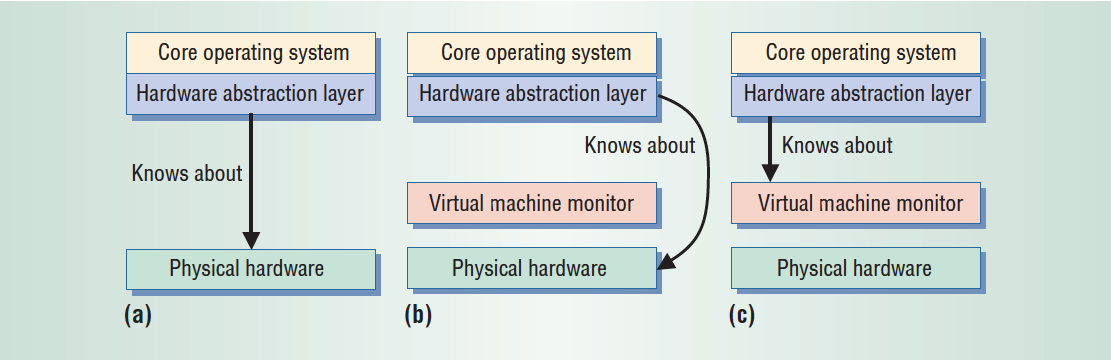
\includegraphics[width=1.0\textwidth]{paravirtualizacion}
\caption{Comparación de arquitectura de sistemas: (a) En un sistema operativo convencional, la capa de abstracción de hardware es la único subsistema del sistema operativo con conocimiento del hardware físico subyacente. (b) Un VMM tradicional expone una replica no modificada de la arquitectura del hardware físico. (c) Un VMM paravirtualizado expone una arquitectura modificada de hardware. Tomado de \cite{whitaker}.}
\end{figure}

En la paravirtualización, el hardware de la máquina física no es simulado en el sistema operativo de la máquina virtual. Se pasa el uso de una interface de programación incorporada que la aplicación puede utilizar para tomar los requisitos del sistema operativo modificado de la máquina virtual.


Para que la virtualización funcione:
Cualquier instrucción peligrosa, que ponga en riesgo la virtualización, tiene que ser privilegiada. Para poner el hardware verdadero en modo no privilegiado para que llegue el VMM y arregle esto. El 386 no cumplia esto. Habian ciertas instrucciones que eran privilegiadas y que no eran tomadas por el VMM.

En el artículo \emph{An old idea: x86 hardware virtualization} de Michal Necasek (\url{http://www.os2museum.com/wp/an-old-idea-x86-hardware-virtualization/}) se expone la situación del momento. A continuación un extracto del artículo:

\textit{The advantages of virtualization were obvious to anyone familiar with IBM's VM/370 system. Older operating systems and applications could be kept running on upgraded hardware, while new operating systems could be incrementally tested in a production environment. Best of all, multiple operating systems could run on the a host system at the same time.}

\textit{With the 386, Intel finally had a processor architecture comparable to mainframe CPUs. Unfortunately hardware support for virtualization was restricted to 8086 systems, as noted above. Virtualizing a 32-bit protected-mode system was not practical.}

\textit{One of the nastier issues was caused by segmentation and GDT/LDT (Global/Local Descriptor Table) usage. A hypervisor could not let a guest operating system manage its descriptor tables (because the guest could overwrite the hypervisor’s memory), yet instructions to store descriptor register values could not be trapped. A guest OS could therefore read true descriptor register values, quite possibly not what it had written.}

\textit{These issues could be avoided by code scanning and patching, but at the cost of high complexity and a significant performance loss. The overhead would likely have made virtualization unattractive.}

\paragraph{}Una de solución a esto fue propuesto por Kevin Smith en su artículo \emph{Virtualizing the 386} (\url{http://www.unz.org/Pub/ProgrammersJournal-1988may-00046})

\textit{The solution was in many ways similar to what Intel implemented in VT-x nearly 20 years later. At the same time it’s also much simpler, primarily because the 386 was a far simpler CPU than the Pentium 4 class processors which first supported VT-x.}

\textit{Smith suggested ``protected normal'' and ``protected VM'' processor modes, much like the root and non-root VMX operation in VT-x. Rather than creating completely new data structures, Smith's design simply extended the existing TSSs (Task State Segments) to store additional information.}

\subsection{Ventajas y desventajas de máquinas virtuales}
Ventajas
\begin{itemize}
 \item Cada máquina esta totalmente aislada de las otras.
 \item Se puede correr cualquier programa.
 \item Protección del sistema operativo.
 \item Provisionamiento de software.
\end{itemize}


Desventajas
\begin{itemize}
    \item Son mas lentas
    \item Hay que tener muchos recursos para tener varias máquinas virtuales.
\end{itemize}


\begin{thebibliography}{9}
    
    \bibitem[WHITAKER et al.]{whitaker} A. Whitaker, R. S. Cox, M. Shaw and S. D. Gribble, \textit{Rethinking the design of virtual machine monitors} in Computer, vol. 38, no. 5, pp. 57-62, May 2005.
    
\end{thebibliography}    
       

\end{document}

















